%% Settings for single-side (simplex) printing
% Margins: left 40mm, right 25mm, top and bottom 25mm
% (but beware, LaTeX adds 1in implicitly)
\documentclass[12pt,a4paper]{report}
\setlength\textwidth{145mm}
\setlength\topmargin{0mm}
\setlength\headsep{0mm}
\setlength\headheight{0mm}
% \openright makes the following text appear on a right-hand page
\let\openright=\clearpage



\usepackage[utf8]{inputenc}
\usepackage{graphicx}
\graphicspath{{../graphs/}}

%% Prefer Latin Modern fonts
\usepackage{lmodern}

\begin{document}
	
	\begin{figure}[h]	
		\centering	
		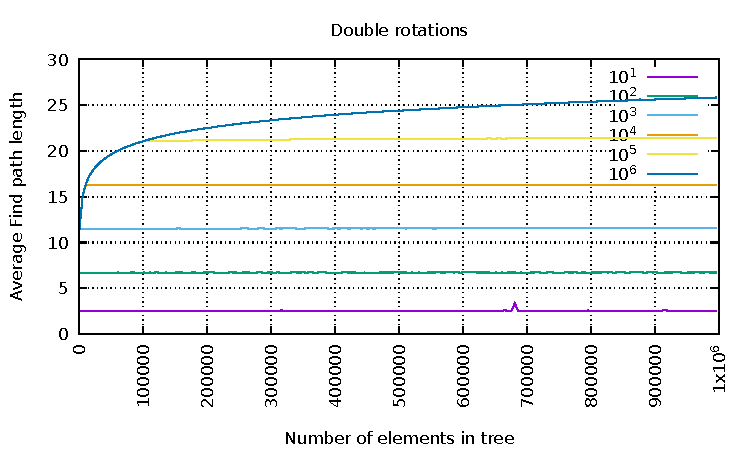
\includegraphics[scale=0.75]{graph_1}		
	\end{figure}

Na prvním grafu můžeme vidět dva zajímavé úkazy. Předně, pro množinu, která je vždy $>=$ velikosti stromu ($10^6$), tj. v které se v průměru mohou objevit a objeví všechny prvky stromu délka logaritmicky roste celou dobu. 

Druhak, pro množiny menší se růst zastaví právě na velikosti stormu. Jakmile totiž dojde vysplejování prvků z vyhledávané množiny k vrcholu, což nastane při jejich prvním vyhledání, tak nám na ostatních prvcích ve stromě  nezáleží. Je tedy jedno kolik jich tam je. Každé další vyhledání prvků za dané množiny bude rozumně rychlé neb všechny jsou a zůstanou (díky povaze operace splay) blízko kořeni. 

Tento jev je pozorovatelný zejména u množiny velikosti $10^5$ (zastavení růstu průměrné délky vyhledávání na stromu o $100 000$ prvcích) a - byť méně viditelně - se projevuje u i množiny velikosti $10^4$, která v první desetině prvního chlívečku osy $x$, tedy do stromu o $10 000$ prvcích, také roste.

	\begin{figure}[h]	
		\centering	
		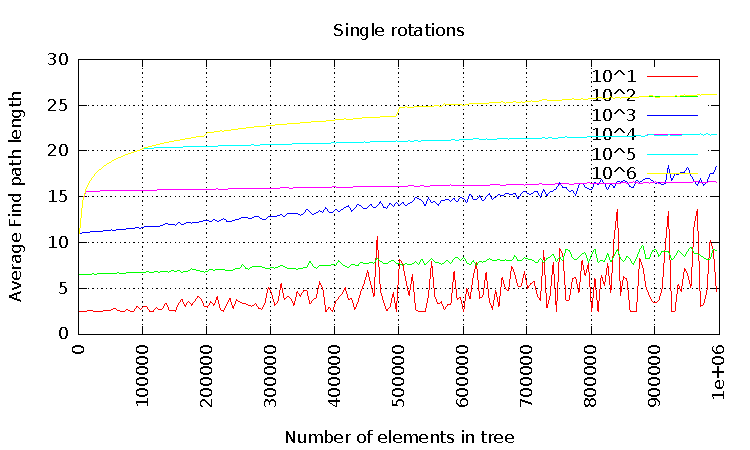
\includegraphics[scale=0.75]{graph_2}		
	\end{figure}

V případě splayování pouze pomocí jednoduchých rotací se projevují také dva zajímavé fenomény. Zejména pro malé vyhledávané množiny mají průměry  daleko větší rozptyl. To je způsobeno tím, že - na rozdíl od dvojitých rotací - záleží na tom, jaké prvky se do dané množiny dostanou. Jak následně ukáže sekvenční test, tak špatná kombinace prvků ve špatném pořadí (splayování prvků v sestupném pořadí) může způsobit průměrnou délku velikosti až poloviny počtu prvků ve stromě. Kvůli tomu pro určité vyhledávací podmonožiny s určitým pořadím může být průměr výrazně horší než u varianty s dvojitými rotacemi.

Ze stejného důvodu, že jednoduché rotace neudržují strom "vyvážený" a některé vrcholy posouvají dolů více než dvojité, se také průměrná délka s velikostí stromu postupně zvyšuje a nezastaví se jako u dvojitých. I když máme omezenou množinu, tak si celou nikdy nevytáhneme ke kořeni. Každé splayování ke kořeni jen s pomocí jednoduchých rotací totiž může ostatní vrcholy od kořene vzdálit. 

	\begin{figure}[h]	
		\centering	
		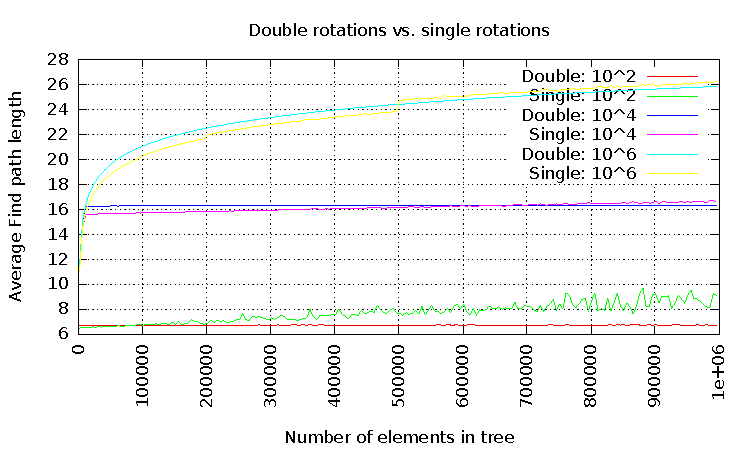
\includegraphics[scale=0.75]{graph_3}		
	\end{figure}

Třetí graf pouze ukazuje výše zmíněné fenomény vůči sobě. Je na něm jasně vidět, že dvojitým rotacím průměrná délka od jisté velikosti stromu nestoupá a její křivka je výrazně hladší. 


	\begin{figure}[h]	
		\centering	
		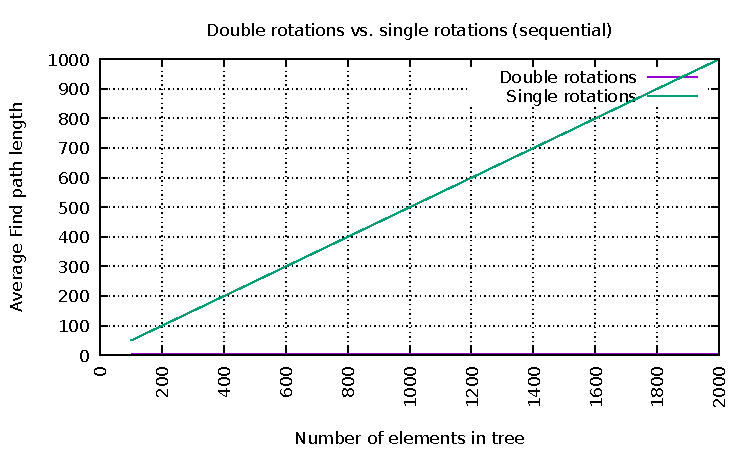
\includegraphics[scale=0.75]{graph_4}		
	\end{figure}

Výše popsané "zhoršující se" chování splay stromu používajícího pouze jednoduché rotace nejlépe ukazuje poslední graf. Na něm je jasně vidět, že na specifických datech může být průměrná délka při findu až poloviční počtu prvků ve stromě. Splay strom korektně využívající dvojité rotace tímto problémem netrpí a udržuje si víceméně konstantní průměrnou délku. 

\end{document}